\section{2D Airfoils}
% The NACA2409 airfoil implies camber: $h=\sfrac{2}{100}\,l$, max thickness occurs at $\sfrac{4}{10}\,l$ from the LE, and max thickness: $t=\sfrac{09}{100}\,l$.
First digit is max camber in hundredths of chord, second digit is the location of max camber along the chord from the leading edge in tenths of chord, last two digits give the maximum thickness in hundredths of chord. For \textit{NACA 2412}: the maximum camber is $0.02c$ located at $0.4c$ from the leading edge, and the maximum thickness is $0.12c$.
\subsection*{Flow around a sharp edge}
For any angle, $\eta$:\\
$\phi=-Br^{\sfrac{\pi}{\eta}}\cos\left(\frac{\pi\theta}{\eta}\right)$\\
$\psi=Br^{\sfrac{\pi}{\eta}}\sin\left(\frac{\pi\theta}{\eta}\right)$\\
$V_r=\frac{\pi}{\eta}Br^{(\sfrac{\pi}{\eta}-1)}\cos\left(\frac{\pi\theta}{\eta}\right)$\\
$V_\theta=-\frac{\pi}{\eta}Br^{(\sfrac{\pi}{\eta}-1)}\sin\left(\frac{\pi\theta}{\eta}\right)$
\subsection*{Kutta condition}
For a 2D body with a sharp trailing edge, there will be a circulation $\Gamma$ such that the rear stagnation point is always at the trailing edge (TE).
% For an airfoil of a given gemoetry and angle of attack, there is a unique $\Gamma$.
A starting vortex generates the CW $\Gamma$ due to boundary layer separation.
The Kutta condition does not need to be satisfied at the LE as the LE in airfoils is always a blunt edge.
% \subsection*{General airfoil nomenclature}
% The max camber is designated $h$, the leading and trailing edge and abbreviated LE and TE, the max thickness is designated $t$. For a symmetric airfoil $h=0$, for asymmetric $h\neq0$. The National Advisory Committee of Aeronautics (NACA) use the following \textit{NACA XYZZ} where X is the camber as a percent of the chord length, Y is the distance of the max camber from the leading edge in terms of the chord length, and ZZ is the thickness as a percent of the chord length.\\


\subsection*{Joukowski Transformation}
$x=\left(r'+\frac{b^2}{r'}\right)\cos\theta'\hfill y=\left(r'-\frac{b^2}{r'}\right)\sin\theta'$\\
$b$ arbitrary, prime notation means $r$ and $\theta$ are taken from cylnder domain.
\subsection*{Flat-plate airfoil (symmetric, zero-thickness)}
Using a cylinder of radius $b$ ($r'=b$)\\
$x=2b\cos\theta',\,\,y=0\quad \text{for } 0\leq\theta'\leq2\pi$\\
$c=4b\hfill h=0\hfill t=0$\\
$\sin\beta=\frac{\Gamma}{4\pi V_\infty R}=\frac{\Gamma}{4\pi V_\infty b}$\\
$\Gamma = \pi V_\infty c\sin\alpha$\\
$L'=\pi\rho V_\infty^2 c\sin\alpha$\\
$c_l=\frac{L}{\sfrac{1}{2}\rho V_\infty^2 c}=2\pi\sin\alpha\approx2\pi\alpha$\\
% $C_P=1-\frac{V_\theta^2\vline_{r=R=b}}{V_\infty^2}$\\
$C_p=1-4\left[\sin(\theta-\alpha)+\sin\alpha\right]^2$
\subsection*{Cambered, thin airfoil (circular arc)}
$\Gamma=4\pi V_\infty R\sin\left(\alpha+\frac{m}{b}\right)$\\
$L'=4\rho\pi V_\infty^2 R\sin\left(\alpha+\frac{m}{b}\right)$\\
$c_l=2\pi\frac{R}{b}\sin\left(\alpha+\frac{m}{b}\right)\approx2\pi\left(\alpha+\frac{2h}{c}\right)$
\subsection*{Symmetric, finite thickness airfoil}
Max thickness: $t=3\sqrt{3}\epsilon$\hfill\text{(at $x=-b$)}\\
$\Gamma=4\pi V_\infty R\sin\alpha$\\
$L'=4\pi\rho V_\infty^2 R\sin\alpha$\\
Since $R=b+\epsilon$ and $l=4b$:\\
$L'=4\pi\rho V_\infty^2\left(\frac{c}{4}+\frac{t}{3\sqrt{3}}\right)\sin\alpha$\\
$c_l\approx2\pi\left(1+\frac{4}{3\sqrt{3}}\frac{t}{c}\right)\alpha$
\subsection*{Joukowsky airfoil}
$\Gamma=\pi V_\infty c\left(1+\frac{4}{3\sqrt{3}}\frac{t}{c}\right)\left(\alpha+\frac{2h}{c}\right)$\\
$c_l=2\pi\left(1+\frac{4}{3\sqrt{3}}\frac{t}{c}\right)\left(\alpha+\frac{2h}{c}\right)$
\subsection*{Lift curve}
All symmetric airfoils, $c_l=0$ at $\alpha=0$. Thickness increases slope of lift curve.\\
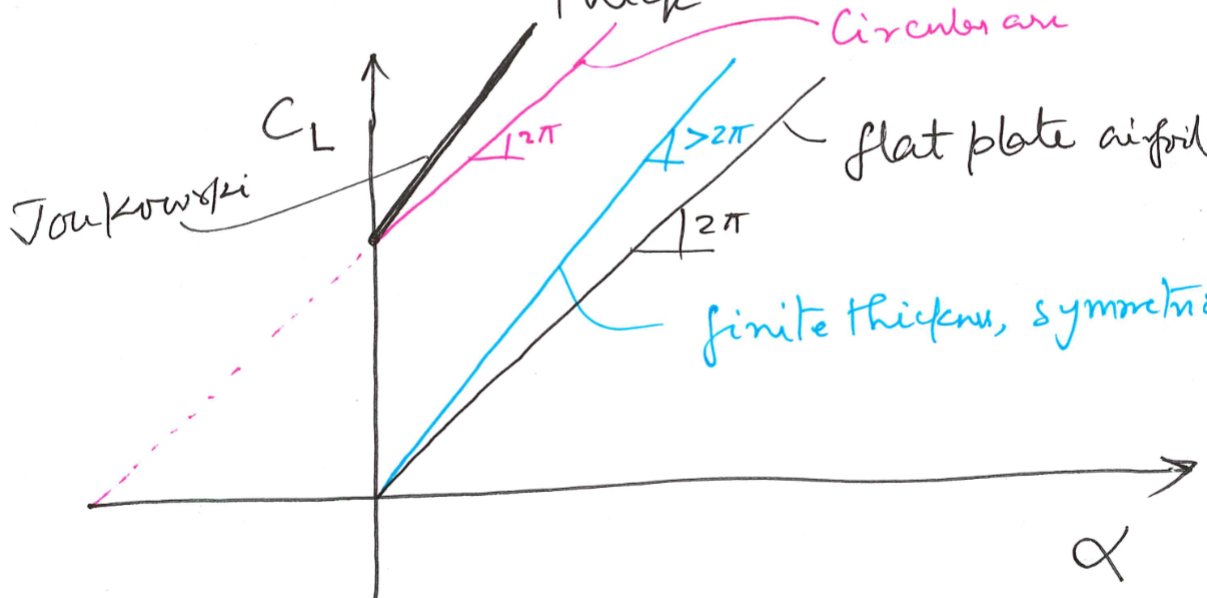
\includegraphics[width=140pt]{images/joukowski chart.png}